% !TeX encoding   = UTF-8
% $Header$

\documentclass[t,14pt,mathserif]{beamer}

% This file is a solution template for:

% - Talk at a conference/colloquium.
% - Talk length is about 20min.
% - Style is ornate.



% Copyright 2004 by Till Tantau <tantau@users.sourceforge.net>.
%
% In principle, this file can be redistributed and/or modified under
% the terms of the GNU Public License, version 2.
%
% However, this file is supposed to be a template to be modified
% for your own needs. For this reason, if you use this file as a
% template and not specifically distribute it as part of a another
% package/program, I grant the extra permission to freely copy and
% modify this file as you see fit and even to delete this copyright
% notice. 


% Copyright 2012 by Aécio S. R. Santos <aecio.solando@gmail.com>.
%
% In principle, this file can be redistributed and/or modified under
% the terms of the GNU Public License, version 2.
%
% However, this file is supposed to be a template to be modified
% for your own needs. For this reason, if you use this file as a
% template and not specifically distribute it as part of a another
% package/program, I grant the extra permission to freely copy and
% modify this file as you see fit and even to delete this copyright
% notice. 

% Redefins a fonte
\usepackage{helvet}

% Define some colors...
\definecolor{titlecolor}{rgb}{0, 0.37, 0.59}
\definecolor{lightblue}{rgb}{.0, .68, .84}
\definecolor{black}{rgb}{0, 0, 0}
\definecolor{gray}{rgb}{0.3, 0.3, 0.3}

% Remove these comments for green color scheme
%\definecolor{titlecolor}{rgb}{0, 0.5, 0.48}
%\definecolor{lightblue}{rgb}{0.2,0.2,0.7}

% Define color of alert text
\setbeamercolor{alerted text}{fg=lightblue}

% Define tamanho das fontes
\setbeamerfont{frametitle}{parent=structure,size=\Large}
\setbeamerfont{framesubtitle}{parent=frametitle,size=\footnotesize}
\setbeamerfont{itemize/enumerate body}{size=\fontsize{16pt}{17.6pt}}
\setbeamerfont{itemize/enumerate subbody}{size=\fontsize{14pt}{15,4pt}}
\setbeamerfont{itemize/enumerate subsubbody}{size=\footnotesize}

% Redefine a fonte do titulo da capa como negrito
%\setbeamerfont{title}{size=\Large, series=\bfseries}

% Redefine cover title color
\setbeamercolor{title}{fg=titlecolor}

% Redefine title color
\setbeamercolor{frametitle}{fg=titlecolor}

% Uncomment to redefine bullets with round format
%\useinnertheme[shadow]{rounded}
%\setbeamertemplate{blocks}[rounded][shadow=\beamer@themerounded@shadow]
%\setbeamertemplate{items}[ball]

% Redefine bullets color
\setbeamercolor*{item}{fg=lightblue}

% Redefine spacing of left margin of bullets
\setlength{\leftmargini}{1.3em}
\setlength{\leftmarginii}{1em}
\setlength{\leftmarginiii}{1em}

% Redefine space between of items in 'itemize' enviroment
\newlength{\wideitemsep}
\setlength{\wideitemsep}{\itemsep}
\addtolength{\wideitemsep}{0.25pt}
\let\olditem\item
\renewcommand{\item}{\setlength{\itemsep}{\wideitemsep}\olditem}

% Redefine space before a nested itemize
\makeatletter
\def\@listii{\leftmargin\leftmarginii
              \topsep    0.9ex
              \parsep    0\p@   \@plus\p@
              \itemsep   \parsep}
\makeatother


% Redefine width of text area margins
\setbeamersize{text margin left=1em,text margin right=1em}

% Define summary items depth
\setcounter{tocdepth}{2}

% Redefine styles of frames' title
\setbeamertemplate{frametitle} {
  \vspace{0.2cm}
  \ifbeamercolorempty[bg]{frametitle}{}{\nointerlineskip}%
  \begin{beamercolorbox}[]{frametitle}
    \ifbeamercolorempty[bg]{frametitle}{}{\nointerlineskip}%
    \usebeamerfont{frametitle}{%
      \strut\insertframetitle\strut\par%
    }
    {%
      \ifx\insertframesubtitle\@empty%
      \else
  \usebeamerfont{framesubtitle}\usebeamercolor[fg]{framesubtitle}\insertframesubtitle\strut\par
      \fi
      \vspace{-.9cm}%
      {
  \textcolor{gray} {\rule[5pt]{\linewidth}{.5pt}\vspace{-8pt}}
      }
    }%  
    \vskip-0.5ex%
    \if@tempswa\else\vskip-.9cm\fi
  \end{beamercolorbox}%
  \vspace{0.2cm}
}

% Removes navigation bar
\beamertemplatenavigationsymbolsempty 

% Redefine footline to show only slide number
\setbeamertemplate{footline}{
  \begin{beamercolorbox}[wd=1\paperwidth,ht=2.25ex,dp=1ex,right]{date in head/foot}%
    %\hfill
    \insertframenumber{}                             % Only current slide number
    %\insertframenumber{} / \inserttotalframenumber  % Current slide number and total of slides
    \hspace{2ex} 
  \end{beamercolorbox}
}

%\usepackage[brazil]{babel}
\usepackage[english]{babel}

\usepackage{graphicx}	%Package para figuras
% or whatever

\usepackage[utf8]{inputenc}
% or whatever

\usepackage{times}
\usepackage[T1]{fontenc}
\usepackage{tabularx}
\usepackage{multirow}
\usepackage{adjustbox}
\usepackage{array}
%\usepackage[cmex10]{amsmath}
% Or whatever. Note that the encoding and the font should match. If T1
% does not look nice, try deleting the line with the fontenc.

\newcommand{\semitransp}[2][35]{\color{fg!#1}#2}

\title[] % (optional, use only with long paper titles)
{Um Estudo de Ferramentas de Suporte de Problemas de Software}

\subtitle {Semana da Pós 2016}

\author[] % (optional, use only with lots of authors)
{Vagner Clementino\\%~\inst{1}% 
	\and Rodolfo Resende - Orientador%\inst{1}%
	}
% - Give the names in the same order as the appear in the paper.
% - Use the \inst{?} command only if the authors have different
%   affiliation.

\institute[] % (optional, but mostly needed)
{
  %\inst{1}%
  Departamento de Ciência da Computação\\
  Universidade Federal de Minas Gerais(UFMG)\\
  
  %\and
   %\inst{2}%
   %Departamento de Ciência da Computação\\
   %Universidade Federal de Minas Gerais(UFMG)\\

  }
% - Use the \inst command only if there are several affiliations.
% - Keep it simple, no one is interested in your street address.

\date[2016/06/14] %o(optional, should be abbreviation of conference name)
%{Software Quality and Measurement 2015-1 \\Prof. Eduardo Figueiredo}
% - Either use conference name or its abbreviation.
% - Not really informative to the audience, more for people (including
%   yourself) who are reading the slides online

\subject{Software Engineer}
% This is only inserted into the PDF information catalog. Can be left
% out. 



% If you have a file called "university-logo-filename.xxx", where xxx
% is a graphic format that can be processed by latex or pdflatex,
% resp., then you can add a logo as follows:

% \pgfdeclareimage[height=0.5cm]{university-logo}{university-logo-filename}
% \logo{\pgfuseimage{university-logo}}



% Delete this, if you do not want the table of contents to pop up at
% the beginning of each subsection:
\AtBeginSubsection[]
{
  \begin{frame}<beamer>{Outline}
    \tableofcontents[currentsection,currentsubsection]
  \end{frame}
}


% If you wish to uncover everything in a step-wise fashion, uncomment
% the following command: 

%\beamerdefaultoverlayspecification{<+->}

\expandafter\def\expandafter\insertshorttitle\expandafter{%
  \insertshorttitle\hfill%
  \insertframenumber\,/\,\inserttotalframenumber}

\setbeamertemplate{caption}[numbered]
\setbeamertemplate{bibliography item}{\insertbiblabel}
\begin{document}

\begin{frame}
  \titlepage
\end{frame}

\begin{frame}{Agenda}
  \tableofcontents
  % You might wish to add the option [pausesections]
\end{frame}


% Structuring a talk is a difficult task and the following structure
% may not be suitable. Here are some rules that apply for this
% solution: 

% - Exactly two or three sections (other than the summary).
% - At *most* three subsections per section.
% - Talk about 30s to 2min per frame. So there should be between about
%   15 and 30 frames, all told.

% - A conference audience is likely to know very little of what you
%   are going to talk about. So *simplify*!
% - In a 20min talk, getting the main ideas across is hard
%   enough. Leave out details, even if it means being less precise than
%   you think necessary.
% - If you omit details that are vital to the proof/implementation,
%   just say so once. Everybody will be happy with that.

\section{Contexto}

\begin{frame}{Contexto}
	
	\begin{itemize}
		\item Dentro do ciclo de vida do software o processo de manutenção tem papel fundamental.
		\item Devido ao seu alto custo, em alguns casos chegando a 60\% do total \cite{kaur2015review}, sua importância vêm sendo considerada tanto pela comunidade científica quanto pela indústria.
	\end{itemize}
  
  
	
\end{frame}

\begin{frame}{Contexto}
	
	\begin{itemize}
		\item A manutenção de software pode ser dividida em \textit{Corretiva, Adaptativa, Perfectiva e Preventiva} \cite{Lientz:1980:SMM:601062,159342}.
		\item A \textit{ISO 14764} \cite{1703974} agrupa os tipos de manutenção em um único termo denominado \textit{Requisição de Mudança - Modification Request (RM)}.
	\end{itemize}
	
	
	
\end{frame}


\section{Motivação}

\begin{frame}{Motivação}
	
	\begin{itemize}
		\item Gerenciar as atividades de manutenção e seus respectivos artefatos possui um alto custo.
		\item Neste contexto, as Ferramentas de Suporte de Problemas de Software ou Sistemas de Controle de Demandas (Issue Tracking Systems) possuem um papel fundamental.
			\begin{itemize}
				\item Facilitam o gerenciamento das MR's
				\item Centralizam a comunicação entre os diversos interessados (stakeholders)
			\end{itemize}
	\end{itemize}
	
	
	
\end{frame}

\begin{frame}{Ferramentas de Suporte de Problemas de Software}
	
		\begin{figure}[hbtp]
			\centering
			
\includegraphics[scale=.3]{../img/issue-tracking-sytem.png}
		\end{figure}
	
	
	
\end{frame}

\begin{frame}{Motivação}

	\begin{itemize}
		\item A utilização de  ``demanda'' parece estar distante das necessidades práticas dos projetos, especialmente no ponto de vista dos desenvolvedores \cite{Baysal:2013:SAP:2486788.2486957}.
		\item Apesar da crescente importância dos SCD's estes sistemas aparentemente não estão atendendo as necessidades dos diversos interessados(stakeholders)
		\item Diversas extensões (plugins) estão sendo propostas na literatura \cite{101186,Thung:2014:BIT:2635868.2661678,Kononenko:2014:DED:2591062.2591075}.
	\end{itemize}	
	
\end{frame}


\section{Objetivo}

\begin{frame}{Objetivo}
	
	\begin{itemize}
		\item Estudar as Ferramentas de Suporte de Problemas de Software visando:
		  
			\begin{itemize}
				\item \textit{Entender} os requisitos básicos deste tipo de ferramenta
				\item \textit{Mapear} as extensões para FSPS que estão sendo propostas na literatura
				\item \textit{Avaliar} sobre o ponto de vista dos profissionais envolvidos em manutenção  a situação atual dos FSPS
				\item \textit{Propor} novas extensões para os FSPS
			\end{itemize}
		
	\end{itemize}	
	
\end{frame}

\section{Metodologia}
\begin{frame}{Metodologia}
	\begin{itemize}
		\item Mapeamento Sistemático da Literatura \cite{kitchenham2007guidelines}
		\item Caracterização de Requisitos das Ferramentas de Suporte de Problemas de Software (FSPS)
		\item Pesquisa (Survey) com os desenvolvedores \cite{wohlin2012experimentation}
		\item Desenvolvimento de extensões para as FSPS's
	\end{itemize}
\end{frame}

\section{Resultados}

\begin{frame}{Mapeamento Sistemático da Literatura}
	
	\begin{itemize}
		\item Situação: Feito	
    \end{itemize}
	
	\begin{figure}[hbtp]
		\centering
		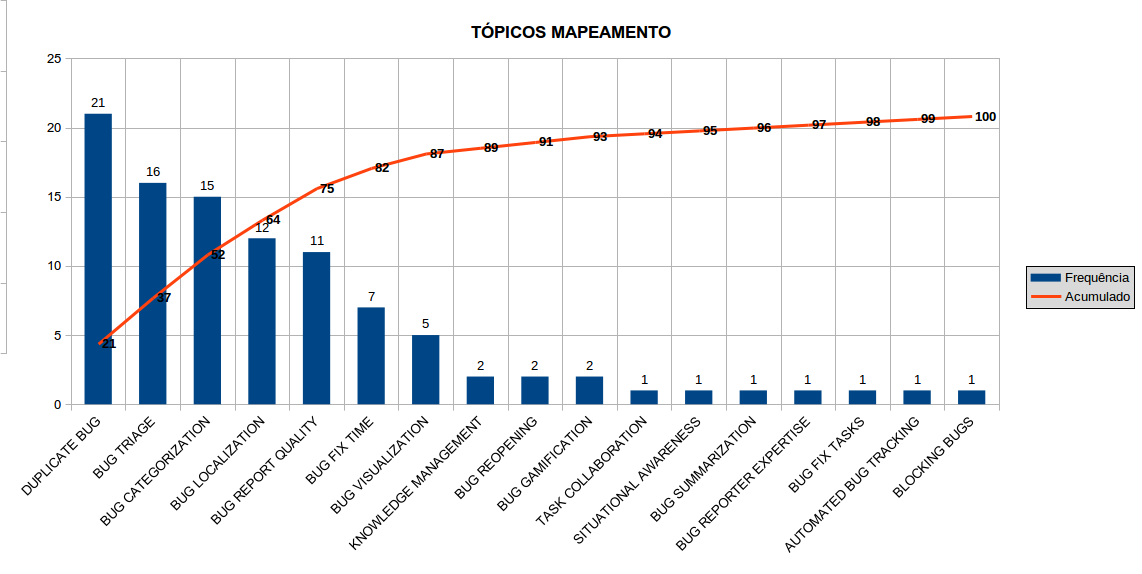
\includegraphics[scale=.39]{../img/mapeamento.png}
	\end{figure}
		
\end{frame}

\begin{frame}{Caracterização de Requisitos das FSPS}
		\begin{itemize}
			\item Situação: Em andamento
			\item Resultados Parciais:
				\begin{itemize}
					 \item CRUD dos problemas
					 \item CRUD de interessados (desenvolvedores, usuários, gerentes de projeto e etc)
					 \item Regras relacionando Problemas vs Interessados
		             \item Classificação (Prioridade e Severidade)				
				\end{itemize}
	    \end{itemize}
\end{frame}

\begin{frame}{Survey com os desenvolvedores}
		\begin{itemize}
			\item Situação: Em andamento
			\item Atividades:
			\begin{itemize}
				\item Planejamento do Survey (Feito)
				\item Ferramenta de Coleta (Em andamento)
				\item "Survey Piloto" (Em andamento)					
			\end{itemize}
		\end{itemize}
\end{frame}


\begin{frame}{Dúvidas?}

	\begin{figure}[hbtp]
		\centering
	
\includegraphics[scale=1]{../img/questions.jpg}
	\end{figure}
	

\end{frame}


\begin{frame}[allowframebreaks]
   \frametitle{References}
   \bibliographystyle{IEEEtranS}
   \bibliography{IEEEfull,semana-da-pos-vagner-clementino}
\end{frame}

\end{document}
	